
\documentclass[11pt, a4paper]{article}
\usepackage{parselines} 
\usepackage{graphicx}
\usepackage{helvet}
\usepackage[utf8]{inputenc}
\renewcommand\familydefault{\sfdefault}
\usepackage{pgfgantt}       % Pour les diagrammes de Gantt
\usepackage{pdflscape}
\usepackage{url}
\usepackage{makecell}
\usepackage{wrapfig}
\usepackage{xcolor}
\usepackage{listings}
\usepackage{amsfonts}
\usepackage{multicol}
\usepackage{mathtools}
\usepackage{amsmath}
\usepackage{float}
\newcommand{\bigzero}{\mbox{\normalfont\Large\bfseries 0}}
\newcommand{\rvline}{\hspace*{-\arraycolsep}\vline\hspace*{-\arraycolsep}}

\usepackage[linesnumbered,ruled,vlined]{algorithm2e}
\usepackage[colorlinks=true,hyperfootnotes=false,citecolor=blue]{hyperref}
\usepackage[capitalise]{cleveref}
\usepackage{siunitx}
\usepackage{todonotes}
\usepackage{cite}
\usepackage{comment}
\usepackage{booktabs}
\usepackage{multirow}
\usepackage{tabularray}
\UseTblrLibrary{booktabs}
\usepackage{caption}
\usepackage{setspace}

\usepackage{geometry}
\usepackage{tabularx}
\usepackage{enumitem}
\usepackage[table, dvipsnames]{xcolor}
\usepackage[utf8]{inputenc}
\usepackage[T1]{fontenc}
\usepackage{lmodern}
\usepackage{amsmath}

\pagestyle{empty}

\geometry{a4paper, margin=1in}

\ganttset{group/.append style={orange},
milestone/.append style={red},
progress label node anchor/.append style={text=red}}

\usepackage{multicol}
\usepackage{titlesec}

\titleformat{\section}{\large\bfseries}{\thesection}{1em}{}
\titlespacing*{\section}{0pt}{1ex}{1ex}

\usepackage{tikz}
\usetikzlibrary{shapes.geometric, arrows}
\tikzstyle{startstop} = [rectangle, rounded corners, minimum width=3cm, minimum height=1cm,text centered, draw=black, fill=red!30]
\tikzstyle{process} = [rectangle, minimum width=3cm, minimum height=1cm, text centered, draw=black, fill=blue!20]
\tikzstyle{arrow} = [thick,->,>=stealth]

\usepackage{enumitem}
\setlist[enumerate]{itemsep=0pt, parsep=0pt, topsep=0pt}
\setlist[itemize]{itemsep=0pt, parsep=0pt, topsep=0pt}



\begin{document}

\title{APP}
\author{Gustavo Banegas}
\date{}
\maketitle

\section{Résumé du Scientifique}
%\begin{enumerate}
%    \item \textbf{Le résumé du scientifique} (3 pages max.) mettant en avant les rubriques suivantes, en lien avec les critères d’évaluation :
%    \begin{itemize}
%        \item \textbf{Présentation} : positionnement, enjeux, objectifs, méthodes, liens avec la stratégie de l’École.
%        \item \textbf{Impacts, retombées et ambitions} : publications, colloques, collaborations, contrat industriel, obtention de financement (ERC, ANR, …).
%    \end{itemize}
%\end{enumerate}


Research in post-quantum cryptography (PQC) has been boosted since 
\href{https://csrc.nist.gov/projects/post-quantum-cryptography/post-quantum-cryptography-standardization/call-for-proposals}
{the National Institute of Standards and Technology (NIST) initiated its PQC standardization project in 2016}. 
The development of PQC schemes typically progresses through four stages:
\begin{enumerate}
\setlength{\itemsep}{0.1pt}
\item \textbf{Mathematical Foundations}: Assessing the computational hardness of underlying mathematical problems;
\item \textbf{Scheme Construction}: Designing cryptographic schemes by leveraging these mathematical problems to create secure trapdoors;
\item \textbf{Algorithm and Prototype Development}: Developing algorithms and coding prototypes, leading to the release of specifications for standard algorithms;
\item \textbf{Deployment and Adoption}: Implementing and widely disseminating the cryptographic schemes.
\end{enumerate}
While many schemes, such as Kyber and Dilithium, have reached stages three or four, 
PQC research remains an active field. There are still numerous open problems and challenges, 
particularly following \href{https://www.nist.gov/news-events/news/2023/07/nist-announces-additional-digital-signature-candidates-pqc-standardization}
{NIST's announcement of new candidates for post-quantum signatures in 2023}. 
Additionally, enhancing efficiency and strengthening implementations against side-channel attacks (SCAs) 
are ongoing priorities. It is also essential to adapt PQC to current applications, including communication protocols, 
hardware security modules (HSMs), and various scenarios such as the Internet of 
Things (IoT) and vehicular communication.

In this research project, I will delineate the challenges that PQC confronts 
in terms of its security evaluation regarding its physical aspects. While presenting these challenges, 
I will put forth a proposal outlining strategies to address the evaluation of security and measurement of 
the countermeasures against side-channel attacks. 

\subsection*{Security Analysis of Post-Quantum Schemes}\label{sec:an}\vspace{-0.1cm}

Cryptosystems face vulnerabilities to SCA, wherein an adversary can deduce 
confidential information from physical observations, such as timing,
electromagnetic emanation, or power consumption, made during the execution of 
sensitive computations. These attacks can be classified as passive, where the a
dversary simply observes leaked information without interfering, or active, 
where faults are intentionally injected to manipulate computations and extract 
secrets. Both types pose serious threats and have been successfully employed 
across various applications, often proving challenging to detect.

Exploring SCA requires specialized equipment and training, as the 
methodologies and countermeasures are highly dependent on the targeted 
cryptosystem. While techniques exist to mitigate these attacks, many are 
intrinsic to specific schemes and lack easy adaptability to others. Consequently, 
securing each implementation demands a unique approach, necessitating 
expertise in both cryptographic engineering and side-channel analysis. 
Unfortunately, the pool of individuals capable of combining these
essential skills remains limited to a select group of professionals.


This research proposal focuses on the security evaluation of post-quantum digital signature schemes selected in the latest NIST call, with a particular emphasis on side-channel analysis (SCA). As cryptographic algorithms transition towards quantum resistance, their resilience to physical attacks remains a critical challenge. The primary objectives of this research are:

\begin{itemize}
    \item \textbf{Evaluation of Side-Channel Attacks}: Analyzing vulnerabilities in selected signature schemes by applying both passive and active side-channel techniques, such as power analysis, fault injection, and electromagnetic analysis.
    \item \textbf{Design of Countermeasures}: Developing robust mitigation strategies tailored to each scheme, including masking, blinding, and fault detection mechanisms.
    \item \textbf{Benchmarking \& Validation}: Assessing the effectiveness of the proposed countermeasures by measuring their security, computational overhead, and feasibility for real-world deployment.
\end{itemize}

This work aligns with the strategic research priorities of the School, particularly in cybersecurity, cryptographic engineering, and embedded system security. It contributes to strengthening expertise in hardware security and advanced cryptographic implementations, reinforcing the School’s position as a leader in post-quantum cryptography research.

\subsection*{Impacts, Outcomes, and Ambitions}

The results of this research will contribute to the broader scientific community by:

\begin{itemize}
    \item \textbf{Publications}: Targeting top-tier cryptography and security conferences/journals such as CHES, EUROCRYPT, CRYPTO, and IEEE Transactions on Information Forensics and Security.
    \item \textbf{Conferences \& Collaborations}: Engaging with academic and industrial partners to disseminate findings, participate in research workshops, and enhance interdisciplinary knowledge exchange.
    \item \textbf{Industrial Impact}: Establishing connections with industry stakeholders, particularly in embedded security and hardware-based cryptographic implementations, to assess the practical adoption of countermeasures.
    \item \textbf{Funding Prospects}: This work is positioned to support funding applications through agencies such as the European Research Council (ERC), the French National Research Agency (ANR), and cybersecurity-focused industrial partnerships.
\end{itemize}



\begin{figure}
\begin{center}
%\resizebox{.5\textwidth}{!}{
%\framebox{
%    \begin{tikzpicture}[node distance=2cm]

        % Nodes
%        \node (start) [startstop] {Research Start};
%        \node (evaluate) [process, below of=start] {Evaluate Side-Channel Attacks (Identify Vulnerabilities)};
%        \node (design) [process, below of=evaluate] {Design Countermeasures (Masking, Blinding, Fault Detection)};
%        \node (benchmark) [process, below of=design] {Benchmark \& Validation (Security, Performance Trade-offs)};
%        \node (end) [startstop, below of=benchmark] {Conclusions \& Future Work};

        % Arrows
%        \draw [arrow] (start) -- (evaluate);
%        \draw [arrow] (evaluate) -- (design);
%        \draw [arrow] (design) -- (benchmark);
%        \draw [arrow] (benchmark) -- (end);

%    \end{tikzpicture}
%    }
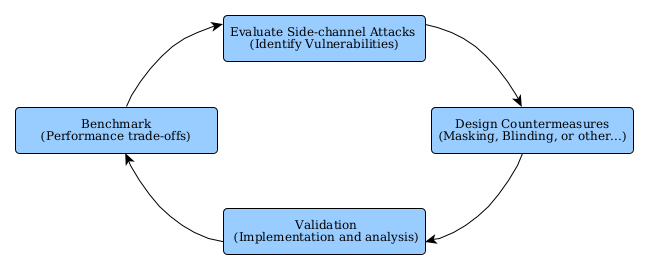
\includegraphics[scale=0.4]{cycle.png}
\caption{Overview of the methdology for the project.}
\end{center}


\end{figure}



%Fortunately, I have honed these skills throughout my career as a researcher and developed hardware 
%proficiency during my tenure at Qualcomm, a leading semiconductor design company. Additionally, I 
%possess knowledge of emerging threats to cryptography, including security analyses leveraging 
%quantum algorithms. Even with NIST moving to 
%\href{https://csrc.nist.gov/Projects/post-quantum-cryptography/round-4-submissions}{Round 4},
%\footnote{\url{https://groups.google.com/a/list.nist.gov/g/pqc-forum/c/fvnhyQ25jUg/m/NJzYDqQBBAAJ}} current 
%submissions are still open to scrutiny, and may be subject to theoretical attacks (where one can break the entire 
%scheme) and side-channel attacks. The whole scientific community can propose attacks and/or improvements for 
%the submissions, to make the schemes more robust. I am therefore particularly interested in doing this.  
%Specifically, I am currently working on \textbf{evaluating security against side-channel attacks} and 
%\textbf{studying quantum algorithms}, to harden PQC algorithms.


Addressing another layer of complexity involves mitigating the countermeasure's impact on speed, code size, or hardware requirements. As part of my \textbf{mid-term goals} and in response to the NIST call for signatures, my ongoing efforts aim to propose efficient countermeasures against these attacks. This represents a vital step in advancing implementation security while maintaining a balance with practical considerations like speed and resource requirements. Fortunately, my background accelerates the comprehension of this process.





Producing new knowledge in this domain aligns with the objectives of the new cybersecurity 
master's program at École Polytechnique de Paris, which aims to equip students with advanced 
expertise in cryptographic security, hardware security, and side-channel analysis. By fostering 
research and innovation in these critical areas, the program contributes to the development of 
next-generation security professionals capable of addressing emerging threats in cryptography 
and beyond.


\begin{landscape}
\section{Calendrier}
\begin{ganttchart}[%Specs
     y unit title=0.5cm,
     y unit chart=0.7cm,
     vgrid,hgrid,
     title height=1,
%     title/.style={fill=none},
     title label font=\bfseries\footnotesize,
     bar/.style={fill=blue},
     bar height=0.7,
%   progress label text={},
     group right shift=0,
     group top shift=0.7,
     group height=.3,
     group peaks width={0.2},
     inline]{1}{36}
    %labels
    %\gantttitle{A three-years project}{36}\\  % title 1
    \gantttitle[]{2025}{6}                 % title 2
    \gantttitle[]{2026}{12} 
    \gantttitle[]{2027}{12}
    \gantttitle[]{2028}{6}\\              
 %   \gantttitle{Q1}{3}                      % title 3
 %   \gantttitle{Q2}{3}
    \gantttitle{Q3}{3}
    \gantttitle{Q4}{3}
    \gantttitle{Q1}{3}
    \gantttitle{Q2}{3}
    \gantttitle{Q3}{3} 
    \gantttitle{Q4}{3}
    \gantttitle{Q1}{3}
    \gantttitle{Q2}{3}
    \gantttitle{Q3}{3} 
    \gantttitle{Q4}{3}
    \gantttitle{Q1}{3}                      % title 3
    \gantttitle{Q2}{3}    \\
    % Setting group if any
   % \ganttgroup[inline=false]{Group 1}{1}{5}\\ 
    \ganttbar[inline=false]{Selection of candidates}{1}{4}\\
    \ganttbar[inline=false]{Acquiring equipment}{3}{5}\\
    \ganttbar[inline=false]{Evaluation of candidates}{5}{10}\\
    \ganttbar[inline=false]{Development of attacks}{6}{12}\\
    \ganttbar[inline=false, bar/.append style={fill=teal}]{Intership Master M2}{5}{11}\\
    %\ganttbar[inline=false]{Writing of the attack}{10}{11}\\
    \ganttmilestone[inline=false]{1st Publication (Journal)}{13} \\
    \ganttbar[inline=false, bar/.append style={fill=purple}]{Writing application for ERC}{9}{12} \\
    \ganttmilestone[inline=false, milestone/.append style={fill=green}]{Deadline Submittion ERC 2026}{12} \\
    \ganttbar[inline=false]{Development of the countermeasure}{11}{16}\\
    \ganttbar[inline=false]{Implementation of the countermeasure}{13}{19}\\
    \ganttbar[inline=false, bar/.append style={fill=teal}]{Intership Master M2}{13}{19}\\
    \ganttbar[inline=false]{Evaluation of the countermeasure}{16}{19}\\
    \ganttbar[inline=false]{Scentific write of the framework}{15}{22}\\
    \ganttmilestone[inline=false]{2nd publication (CHES)}{20} \\
    \ganttbar[inline=false]{Evaluation of hardware design }{20}{26}\\
    \ganttbar[inline=false]{Prototype of secure hardware}{22}{32}\\
    \ganttbar[inline=false]{Evaluation of secure techniques}{26}{34}\\
    \ganttmilestone[inline=false]{3nd publication (CHES/Eurocrypt)}{35} \\
    %\ganttbar[inline=false]{Preparatiof for the defense}{33}{36}\\
    %\ganttmilestone[inline=false]{PhD Thesis Defense}{36} \\ 
\end{ganttchart}
\end{landscape}


\newpage
\section{CV}
\begin{enumerate}
    \item The scientific summary (maximum 3 pages) highlighting the following sections, in connection with the evaluation criteria:
    \begin{itemize}
        \item \textbf{Presentation:} positioning, challenges, objectives, methods, links with the School's strategy.
        \item \textbf{Impacts, outcomes, and ambitions:} publications, conferences, collaborations, industrial contracts, funding acquisition (ERC, ANR, ...).
    \end{itemize}
    
    \item The timeline detailing the work plan over 3 years (maximum 1 page).
    
    \item The projected budget over 3 years (maximum 1 page). This budget must be realistic, and the Foundation reserves the right to suspend or even terminate the project's funding, particularly in the event of an unjustified failure to comply with the budget.
    
    \item The candidate's CV (maximum 3 pages).
\end{enumerate}

\subsection*{CV}
\medskip


\subsection*{Professional Experience}
\resizebox{\linewidth}{!}{
\begin{tabular}{|c|c|c|c|}
 \toprule
 Start & End &
  Institution & 
 Position and status\\ 
  \midrule
  01/10/2024  & Current & INRIA & ISFP (Cryptography Researcher) \\
  01/06/2022   & 30/09/2024 & Qualcomm & Senior Cryptographer \\
  01/12/2020     & 30/05/2022   & INRIA Saclay & Post Doc \\
  01/11/2019      & 30/11/2020   & Chalmers University of Technology 
                               & Post Doc \\
 01/11/2015      & 12/11/2019   & Technische Universiteit Eindhoven 
                               & Ph.D. Candidate \\
 01/09/2018     & 01/12/2018   & CryptoExperts 
                               & Internship \\
 01/02/2017     & 01/05/2017   & Riscure 
                               & Internship \\
 01/10/2014     & 31/10/2015   & Bry Tecnologia 
                               & Software Engineer  \\   
\bottomrule
\end{tabular}
}



\subsection*{Scientific Responsabilities}
\begin{table}[h]
    \centering
     \caption{Conference Involvement}
    \label{tab:conference_involvement}
    \renewcommand{\arraystretch}{1.3}
    \setlength{\tabcolsep}{10pt}
    \begin{tabular}{l|l}
        \toprule
        \textbf{Role} & \textbf{Conferences and Years} \\
        \midrule
        \multirow{9}{*}{\textbf{Program Committee Member}} & AsiaCCS: 2025 \\
        & Communications in Cryptology: 2025 \\
        & CBCrypto: 2020, 2021 \\
        & CHES: 2022, 2023, 2024 \\
        & Eurocrypt: 2022 \\
        & LatinCrypt: 2023, 2025 \\
        & Asiacrypt: 2023 \\
        & ACNS: 2024 \\
        & PQCrypto: 2025 \\
        \midrule
        \multirow{6}{*}{\textbf{External Reviewer}} & CRYPTO: 2022 \\
        & Asiacrypt: 2018, 2019, 2020, 2021 \\
        & FSE: 2021 \\
        & LatinCrypt: 2021 \\
        & SPACE: 2020 \\
        & PQCrypto: 2018 \\
        \bottomrule
    \end{tabular}
\end{table}

\subsection*{Supervision}
\paragraph{Master Thesis}
~\\
Iggy van Hoof, \textit{Concrete quantum-cryptanalysis of binary elliptic curves}, Eindhoven University of Technology, 2019.

\paragraph{Bachelor Thesis}
~\\
Sigurjon Agustsson, \textit{Montgomery Reduction in RSA}, École Polytechnique, 2021.
~\\
David Brandberg, Lisa Fahlbeck, Henrik Hellstr\"om, Hampus Karlsson, John Kristoffersson, Lukas Sandman, \textit{End-to-end Encrypted Instant Messaging Application}, Chalmers University of Technology, 2020.

\paragraph{Intern at Qualcomm} 
~\\
Liana Koleva, \textit{Vectorization of HQC on RISC-V architecture}, 2023. 


\section*{Selected Publications}

For a full list of publications see: \href{https://scholar.google.com/citations?user=0AIDhMwAAAAJ&hl=fr}{Google Scholar}, 
\href{https://cryptme.in/#publications}{Personal Website} or \href{https://dblp.org/pid/150/9441.html}{DBLP}.

\begin{enumerate}\small
%\item Gustavo Banegas and Ricardo Villanueva-Polanco. On recovering block cipher secret keys in the cold boot attack setting. \textit{Cryptography and Communications}, 2023.
%\item Gustavo Banegas, Valerie Gilchrist, and Benjamin Smith. Efficient supersingularity testing over $\mathbb{GF}(p)$ and CSIDH key validation. \textit{Mathematical Cryptology}, 2(1), 21-35, 2022.
\item Estuardo Alpirez Bock, Gustavo Banegas, Chris Brzuska, Łukasz Chmielewski, Kirthivaasan Puniamurthy, and Milan Šorf. Breaking DPA-protected Kyber via the pair-pointwise multiplication. \textit{ACNS 2024. Lecture Notes in Computer Science}, vol 14584.
\item Gustavo Banegas, Valerie Gilchrist, Anaëlle Le Dévéhat, and Benjamin Smith. Fast and Frobenius: Rational isogeny evaluation over finite fields. \textit{LATINCRYPT 2023. Lecture Notes in Computer Science}, vol 14168.
\item Gustavo Banegas, Daniel J. Bernstein, Fabio Campos, Tung Chou, Tanja Lange, Michael Meyer, Benjamin Smith, and Jana Sotáková. CTIDH: Faster constant-time CSIDH. \textit{IACR Transactions on Cryptographic Hardware and Embedded Systems}, 2021(4):351–387, 2021.
\item Gustavo Banegas, Daniel J. Bernstein, Iggy van Hoof, and Tanja Lange. Concrete quantum cryptanalysis of binary elliptic curves. \textit{IACR Transactions on Cryptographic Hardware and Embedded Systems}, 2021(1):451–472, 2020.
%\item Gustavo Banegas, Paulo S. L. M. Barreto, Edoardo Persichetti, and Paolo Santini. Designing efficient dyadic operations for cryptographic applications. \textit{Journal of Mathematical Cryptology}, 14(1):95–109, 2020.
%\item Bei Liang, Gustavo Banegas, and Aikaterini Mitrokotsa. Statically aggregate verifiable random functions and application to e-lottery. \textit{Cryptography}, 4(4), 2020.
%\item Georgia Tsaloli, Gustavo Banegas, and Aikaterini Mitrokotsa. Practical and provably secure distributed aggregation: Verifiable additive homomorphic secret sharing. \textit{Cryptography}, 4(3):25, 2020.
\item Gustavo Banegas, Paulo S. L. M. Barreto, Brice Odilon Boidje, Pierre-Louis Cayrel, Gilbert Ndollane Dione, Kris Gaj, Cheikh Thiécoumba Gueye, Richard Haeussler, Jean Belo Klamti, Ousmane Ndiaye, Duc Tri Nguyen, Edoardo Persichetti, and Jefferson Ricardini. DAGS: Key encapsulation using dyadic GS codes. \textit{Journal of Mathematical Cryptology}, 12(4):221–239, 2018.
%\item Gustavo Banegas, Ricardo Custódio, and Daniel Panario. A new class of irreducible pentanomials for polynomial-based multipliers in binary fields. \textit{Journal of Cryptographic Engineering}, Online first:1–15, 2018.
%\item Gustavo Banegas and Florian Caullery. Multi-armed SPHINCS+. \textit{ACNS 2023. Lecture Notes in Computer Science}, vol 13907.
%\item Simona Samardjiska, Paolo Santini, Edoardo Persichetti, and Gustavo Banegas. A reaction attack against cryptosystems based on LRPC codes. \textit{LATINCRYPT 2019}, pp. 197–216.
\item Gustavo Banegas and Daniel J. Bernstein. Low-communication parallel quantum multi-target preimage search. \textit{SAC 2017. Lecture Notes in Computer Science}, vol 10719, pp. 325–335.
%\item Gustavo Banegas and Ricardo Villanueva-Polanco. A Fault Analysis on SNOVA. \textit{Cryptology ePrint Archive}, Paper 2024/1883. \url{https://ia.cr/2024/1883}
%\item Gustavo Banegas, Thomas Debris-Alazard, Milena Nedeljković, and Benjamin Smith. Wavelet: Code-based post-quantum signatures with fast verification on microcontrollers. \textit{Cryptology ePrint Archive}, Report 2021/1432. \url{https://ia.cr/2021/1432}
\end{enumerate}
In cryptography, it is common to author list in alphabetical order. We usually follow the cultural statement of \href{https://www.ams.org/profession/leaders/CultureStatement04.pdf}{American Mathematical Society}. 

\subsection*{Teaching}
\textbf{Special Class} (2021) — Universidade Federal de Santa Catarina (Online), Florianópolis, Brazil  
Taught Quantum Computation, Grover's Algorithm, and Shor's Algorithm. ~\\

\textbf{Special Classes} (2020) — Chalmers University of Technology, Gothenburg, Sweden  
Taught various cryptography topics, replacing Prof. Katerina Mitrokotsa:  
\begin{itemize}
\item RSA and Primality Testing  
\item Attacks on Block Ciphers and Intro to PKC  
\item Block Ciphers and Operation Modes  
\item Sigma Protocols  
\end{itemize}

\textbf{Tutor} (2016--2019) — Technische Universiteit Eindhoven, Netherlands  
Tutor for courses including:  
\begin{itemize}
\item Introduction to Cryptology  
\item Basic Mathematics  
\item Algebra and Discrete Mathematics  
\end{itemize}

\subsubsection*{Grants}
\textbf{Marie Skłodowska-Curie ITN} — \href{https://www.ecrypt.eu.org/net/}{ECRYPT-NET Project}  
Fellow PhD (2015–2019).  
~\\ \\
\textbf{Wallenberg WASP Expedition Project} — Massive, Secure, and Low-Latency Connectivity for IoT Applications  
Fellow Researcher (2019–2020).  


\subsection*{Software}

\small
\begin{itemize}
\setlength{\itemsep}{1pt}
    \item \textbf{WAVE}: \href{https://github.com/wavesign/wave}{\texttt{github.com/wavesign/wave}}
    \item \textbf{Wavelet}: \href{https://github.com/wavelet/}{\texttt{github.com/wavelet/}}
    \item \textbf{CTIDH}: \href{http://ctidh.isogeny.org/software.html}{\texttt{ctidh.isogeny.org/software.html}}
    \item \textbf{DAGS Key Encapsulation}: \href{https://github.com/gbanegas/dags_v2}{\texttt{github.com/gbanegas/dags\_v2}}
    \item \textbf{HSS/LMS Hash-Based Signatures}: \href{https://github.com/gbanegas/sphss}{\texttt{github.com/gbanegas/sphss}}
    \item \textbf{More Code}: \href{https://github.com/gbanegas/}{\texttt{github.com/gbanegas/}}
\end{itemize}




\newpage
%\nocite{*}
\bibliographystyle{plain} 
\bibliography{research}   

\end{document}

